\chapter{Detection at colliders and accelerators}\label{chapter:collider}\index{Collider}
Production of DM at accelerators represents  the third possible way in which DM can be searched for and its properties ultimately tested, see fig.\fig{dirindcol}.
The most straightforward interpretation of DM as a thermal relic leads to a testable prediction given in eq.~\eqref{eq:DMrelicmassTeV}:
a DM with order-unity couplings (as is the case for weak gauge interactions) has a TeV-scale mass, while DM is even lighter, if the couplings are smaller. 
This can be tested at particle accelerators -- current and planned colliders are capable of producing particles in this mass range. 
 Even if one allows larger, non-perturbative, couplings, the thermal relic DM must still be lighter than 100 TeV, see eq.\eq{100TeV}, 
and can thus still be a target of possible future colliders. 


However, even if colliders might have already produced DM particles, this by itself is not enough for a discovery. 
Once produced, the DM particle must also be detected, which is not completely straightforward. 
The only unavoidable signature of DM is missing energy (missing transverse energy at hadron colliders) since DM interacts only feebly  with matter and escapes the detector, carrying with it energy and momentum.
This is an indirect and  rather difficult signature, and can be limited by our understanding of the backgrounds.

Specific DM models can also predict signals that are much easier to detect, at colliders or at other accelerator-based experiments. DM may be accompanied by other states, for instance new mediators, that can decay to the SM particles, giving visible imprints in the detectors. 
Such signatures are model-dependent, with a vast literature devoted to them. 
To date, no statistically significant deviations from the SM have been observed, either in missing energy or in visible channels.
Conversely,  a positive signal at colliders would allow to devise dedicated measurements 
to better understand DM using the controlled laboratory environment. 

\medskip

This chapter starts with a focus on `traditional' TeV DM searches at colliders, and then enlarges its scope in later sections. After a quick overview of the basic principles of collider physics in section \ref{sec:collider_summary}, we discuss the main signatures of DM at colliders in section \ref{sec:DMatcolliders}, and compare it with other detection strategies in section \ref{sec:complementarities}. The searches for more general DM models  are covered in section \ref{sec:searches:beam:dumps}. These are mostly accelerator-based, but also cover particle physics experiments in a wider sense and thus even include atomic physics and astrophysics searches when these can probe the same physics. 

\section{A brief summary of collider physics}\label{sec:collider_summary}
High energy physics is strongly affected by what can and cannot be done with collider experiments.
We therefore first briefly summarize the main facts about colliders.


\subsection{Production}
There are two main types of colliders:
\begin{description}
\item {\bf Electron-positron colliders}.
In order to reach high energies, $e^\pm$ are accelerated in circular orbits with radius $R$.
The energy of a circular collider  is limited by the energy losses via Larmor radiation,
$dE/dx = 2 \alpha{\gamma^4}\beta^3/3{R^2}$ 
where $\gamma =E/m_e$ is the Lorentz factor.
  Imposing
 that this equals the maximal energy loss, 
$dE/dx|_{\rm max}$, which one is able to deliver to $e^\pm$ in a given accelerator using electric fields, fixes the maximal energy of an $e^+e^-$ collider:
\beq 
\frac{E_{\rm max}}{m_e}= 
\gamma_{\rm max} \approx  \sqrt[4]{R^2\cdot {dE/dx|_{\rm max}}} \sim 6~10^5\sqrt{\frac{R}{5\km}}\sqrt[4]{\frac{dE/dx|_{\rm max}}{m_ec^2/10\cm}}.\eeq
The last such collider was LEP, that reached center-of-mass energy $\sqrt{s}\approx 200\GeV$ and had a radius $R\approx 4.3$\,km. There are now discussions to build the next version of such a collider with $R\approx 15$\,km and thus a higher energy.
However, since the maximal energy increases only slowly with the circular collider parameters, $R$ and $dE/dx|_{\rm max}$,
the alternative is to build linear $e^+e^-$ colliders.
Their maximal energy is limited by their length $L$ as 
\beq 
E_{\rm max} = L   \left.\frac{dE}{dx}\right|_{\rm max}  = 1\TeV \frac{L}{10\km} \frac{dE/dx|_{\rm max}}{1 \MeV/{\rm cm}}.
\eeq
Attempts to reduce $L$ by devising technologies that allow
much higher values of $dE/dx|_{\rm max}$ are being studied.
Circular muon colliders, if feasible in the future
(muons need to be collimated and accelerated before they decay),
would  reach much higher energies bypassing the energy loss issue thanks to $m_\mu \gg m_e$.

\item  {\bf Hadron colliders} collide protons with protons or with anti-protons (and possibly heavier nuclei with other nuclei).
The $p\bar p$ option leads to a better use of the collision energy, while the $pp$ option has the advantage that the proton beams can be made more intense.
Since $m_p\gg m_e$ the Larmor radiation is negligible in current and past hadron colliders.
Their energy is instead limited because, according to the Lorentz force, 
a strong magnetic field $B$ is needed to circulate 
$p$ or $\bar p$ with high energy $E$ along orbits with radius $R$
(as needed to slowly accelerate them via electric fields):
\beq  E=QRB = 15\TeV \frac{Q}{e}\frac{R}{5{\rm km}}\frac{B}{10\,{\rm Tesla}},
\eeq
where we neglected the mass of $p$ or $\bar p$ compared to $E$.
Magnetic fields exceeding tens of Tesla surpass the atomic electric fields responsible for holding ordinary matter together.
Consequently, their magnetic pressure $\wp \sim B^2/2\mu_0$ is so strong that it causes mechanical devices to break apart.
Furthermore, the highest magnetic fields are obtained by relying on super-conducting materials carrying large currents. Superconductivity is achieved at
low temperatures, and thus requires sophisticated cryogenic systems, lots of energy, and leads to significant time waste whenever a problem arises.

\index{LHC}\index{Collider!LHC}
The LHC $pp$ collider started in 2010 and reached $\sqrt{s}=13.6\TeV$ in 2022.
So far its CMS and ATLAS experiments accumulated an integrated luminosity of about $ 100-200/{\rm fb}$.
The plan for LHC is to enter a high luminosity phase, without raising the collision energy,
until  $\sim 3000/{\rm fb}$ are accumulated around 2035.
A future $pp$ collider with $\sqrt{s}\sim 100\TeV$ is being discussed. Assuming the cost is not prohibitively high, 
it will be built only many decades in the future.

While hadron colliders reach higher energies than electron colliders, 
their physics reach is limited by the fact that
protons are not elementary particles.  This implies that:
a) Elementary quarks and gluons inside protons only contain a variable fraction $x\sim 0.1$ of the total proton momentum, such that each elementary collision has a reduced energy ${\hat{s}} = x_1 x_2 s$.
b) The large cross-section $\sigma(pp)\sim 1/m_\pi^2$, where $m_\pi=0.14$ GeV is the pion mass, produces large QCD backgrounds to the elementary
processes that one would like to investigate, which have much smaller cross sections, $\hat \sigma \sim 1/\hat s$ .
Since the SM backgrounds also contain neutrinos, which are invisible to the LHC experiments just like the DM is, this presents a challenge 
 when looking for missing energy signals.
 
 \item  {\bf Fixed target experiments.} 
 Fixed target experiments are experimentally simpler than the hadron and electron colliders, since one needs to only create one beam, which then collides with the target at rest. Due to its relative simplicity the beam can be made out of protons or electrons, but also out of muons. Another benefit is that beams can be optimised for intensity, so that one can collect large data samples of collisions. On the negative side, the center of mass of the collision, $\sqrt{s}=\sqrt{2 E m_p}$, is much smaller than the energy of the beam $E$ (here $m_p$ is the mass of the proton as a stand-in for the mass of the nucleons in the target material, and we neglected the mass of the particles in the beam). Especially interesting for  dark sector searches  are the so called {\em beam dump} experiments, in which the beam is dumped into a dense block of a heavy material, so that the hadronic cascade is absorbed as fast as possible.
 
\end{description}

Since cross sections for the production of heavy new particles get smaller at higher collision energy, $\hat s$,  intense and collimated
beams are needed to see a statistically significant number of high-energy events.
So far, a relatively large number of SM processes were seen at the highest energies at the LHC, with no significant excesses. This is signaling that DM is either heavier or that it has couplings small enough that it is not being produced in any appreciable quantity.


\subsection{Detection}
A typical particle detector only detects directly the  lightest few particles, which are either stable or long-lived on collider timescales, such that they leave visible imprints:

\begin{itemize}
\item[$\circ$] {\bf Electrons and photons} are seen in electro-magnetic calorimeters. These devices can reliably identify them and measure their
energies with $\approx 1\%$ level precision.

\item[$\circ$] {\bf Muons} appear as almost-stable particles. 
A magnetic field in the external volume of the apparatus allows to identify them, distinguishing between $\mu^+$ and $\mu^-$.
Additionally, their momentum can be measured
from the curvature of their trajectories, provided that their energy is not much larger than 1 TeV.

\item[$\circ$] {\bf Quarks and gluons} appear, in collisions with energy release well above the QCD scale, as jets of hadrons whose momenta
are measured in a dedicated hadronic calorimeter.
 In conjunction with other instruments, this allows for the identification of the main hadrons: $\pi^\pm$, $p$, $n$, $K$,\ldots~By summing their energies, the jet energy can be reconstructed with $\approx 10\%$ uncertainty.
The phase space distributions of the hadrons offer  only limited means to discriminate quarks from gluons.
 A tracker positioned near the production point can identify bottom quarks based on their displaced decays.


\item[$\circ$] {\bf Neutrinos} are inferred indirectly from the fact that they carry away some fraction of the total energy
of the event or, at hadronic colliders, some `transverse energy'
(momentum in the direction transverse to the colliding beams).


\end{itemize}
Heavier particles can be identified via their decay products. For example, a $Z$ boson decaying
into a $\mu^+\mu^-$ pair can be recognised by using their four-momenta $P_{\mu^\pm}$ to calculate the 
invariant mass $M_{\rm inv}^2\equiv(P_{\mu^+} + P_{\mu^-})^2$ and checking that it agrees with $M_Z^2$.
More complicated versions of this basic idea 
allow to devise kinematical variables~\cite{Barr:2003rg} useful for
partially discriminating the missing energy produced by
light particles (such as neutrinos) from the missing energy produced by heavier particles (such as possibly DM).





\section{Dark Matter signals at colliders}\label{sec:DMatcolliders}
Given that DM must be a stable neutral particle, it cannot be singly produced at colliders but rather only in pairs such as DM$+\overline{\rm DM}$  or DM$+$DM, possibly together with extra SM particles.
More complicated DM theories may require three or more DM particles to be produced simultaneously.
The collider energy therefore needs to be at least  $\sqrt{\hat s}>2 M$, in order to be able to produce DM.  Once produced, free DM particles
escape without interacting with the detectors, resulting in a missing energy signal in the same way as neutrinos do.\footnote{Alternatively,
two DM particles produced almost at rest can form a dark bound state, which then decays through the annihilation
of its components into visible states. This only happens in models where DM interacts via light enough particle such that dark bound states can exist.
In these models, scatterings among SM particles can receive a detectable correction from
diagrams where DM appears in loops~\cite{DMboundstatecollider}.}
Such a minimal signal of DM is detectable only if some other visible particle is also produced during the collision,
otherwise the event goes unnoticed.
The visible particles might be produced automatically, e.g.,\ when DM pairs are produced
inside decay chains such as in eq.\eq{SUSYdecaychains}. Otherwise, one needs
to search for rarer events where a photon or a jet is produced together with DM (the so called {\em mono-photon} and {\em mono-jet} signatures).


\subsection{Supersymmetric Dark Matter}\label{sec:SUSYcolliderpheno}\index{Supersymmetry!collider}
The Higgs mass hierarchy problem motivated the presence of a new supersymmetric partner for each SM particle,
with masses below about 1 TeV.
The lightest of such supersymmetric particles (LSP, most probably a neutralino, here denoted as $N$ and elsewhere often as $\chi_0$) 
is a good DM candidate (see section \ref{SUSY}).
This supersymmetric DM scenario was so popular that the word `neutralino' was often used as a synonym for DM,
see, e.g.,\ old reviews in~\cite{otherpastDMreviews}.
Within such a scenario, $pp$ collisions were expected to produce large numbers of 
supersymmetric particles with strong interactions,
gluinos, $\tilde{g}$, and squarks, $\tilde{q}$.
These particles  would ultimately decay into DM, 
possibly through long chains of successive decays, such as
\beq\label{eq:SUSYdecaychains}
pp \to  \tilde g \tilde g,\qquad
 \tilde g \to \bar q\tilde{q} \to \bar q q \chi \to \bar q q \ell \bar \nu N,
 \eeq
where $\chi$ denotes a chargino and $\ell$ a charged lepton.
The decay modes depend on the unknown mass ordering of sparticles.
This scenario predicts a large cross section for
missing energy events accompanied by possibly many leptons and jets.
Many studies focused on special models (such as `CMSSM' - the Constrained Minimal Supersymmetric Standard Model)
and tried to develop general techniques for reconstructing the DM mass and the sparticle masses from 
invariant masses, end-points and other kinematical features of the rich decay chains.

Long decay chains, such as the one in eq.\eq{SUSYdecaychains}, would have been such a distinct experimental signature 
that already a single type of events might have enabled the simultaneous discovery of DM, supersymmetry, and Higgs naturalness
(section~\ref{SUSY}). However, physicists are still waiting for statistically significant excesses of such events.
Nothing like this was observed at the LHC with $\sqrt{s}=13\TeV$ after about $2\times140$/fb of integrated luminosity.


\bigskip

Several other DM signals
have been proposed based on different variants of supersymmetric DM. 
One such possibility is that the LSP is not stable but decays into gravitino DM
(the gravitino is the spin-3/2 supersymmetric partner of the graviton).
If the LSP is electromagnetically charged and/or carries QCD color, and its decay rate is sufficiently slow,
 it would be possible to detect both the LSP charged tracks and the secondary vertices from the LSP decays.

Another possibility is that the LSP has such a long lifetime that it first stops in the detector and then decays only at a much later time,
potentially even after the collider has already been turned off.
Which decay channels dominate depends on the identity of the LSP: a photino would decay into a photon and a gravitino;
a slepton would decay into a lepton and a gravitino, etc.




In light of negative results from the LHC, one hypothesis that has been entertained is that the only light sparticles are the stop $\tilde t$ (relevant for the Higgs mass hierarchy problem) and the DM.
The expected DM signal would be the $pp\to \tilde t \tilde t^*$ production, potentially accompanied by initial-state radiation,
followed by $\tilde t$ decays into DM,
e.g.,\ $\tilde t \to t N$ if $M_{\tilde t} > M + M_t$. 
The correct cosmological DM abundance is obtained for
$M_{\tilde t}- M \approx 35 \GeV$, i.e., in the regime where stop co-annihilations play a pivotal role to explain DM as a thermal relic (see section~\ref{sec:colocoann} below).


\subsection{Colored co-annihilations}\label{sec:colocoann}
A notable DM scenario, especially relevant for DM searches at hadron colliders, is DM accompanied by a dark sector that contains a slightly heavier colored particle, DM$'$~\cite{ColoredCoannihilations}.
For example, in supersymmetric models DM is the lightest neutralino, with mass $M$, 
while a gluino or a squark can be only slightly heavier, with a mass $M' = M + \Delta M$.
In this case, even if ${\rm DM}+{\rm DM}$ annihilations are negligible, the desired DM thermal relic abundance
can be obtained from co-annihilations, see section~\ref{sec:coann}. The excess DM abundance is annihilated away since DM can be converted to DM$'$ 
through scattering on the SM plasma, after which DM$'$ annihilate through sizable
cross sections dictated by QCD,
\beq\label{eq:crisscross}
\sigma({\rm DM}'{\rm DM}'\to gg+q\bar q ) v_{\rm rel}=\dfrac{\pi\alpha_{\rm s}^2}{M_{{\rm DM}^\prime}^2}\times
\left\{
\begin{array}{ll}
\sfrac{7}{27}& \quad\textrm{if DM$'$ is a scalar color triplet,}\\[2mm]
\sfrac{27}{16}& \quad\textrm{if DM$'$ is a  scalar color octet,}\\[2mm]
\sfrac{7}{54}+2/3& \quad\textrm{if DM$'$ is a  fermion color triplet,}\\[2mm]
\sfrac{27}{32}+\sfrac{9}{8}& \quad\textrm{if DM$'$ is a  fermion color octet.}\\
\end{array}
\right.   
\ee
Using the results of section~\ref{sec:coann}, but specializing to the case of co-annihilations in which only 
the colored particles can annihilate, the total DM abundance
$Y=g_{\rm DM} Y_{\rm DM} + g_{{\rm DM} '} Y_{{\rm DM}'}$ is obtained from the effective
annihilation cross section
\be\label{sigmav}
 \sigma_{\rm eff} =
\sigma({\rm DM}'{\rm DM}'\to \textrm{SM})
\times R^2 ,\qquad
R=\frac{g_{{\rm DM}'} Y_{{\rm DM}'}^{\rm eq}}{g_{{\rm DM}} Y_{{\rm DM}}^{\rm eq}+g_{{\rm DM}'} Y_{{\rm DM}'}^{\rm eq}} =
\left[ 1+ \frac{g_{\rm DM}}{g_{{\rm DM}'} }\frac{\exp(\Delta M/T)}{(1+\Delta M/M)^{3/2}}
\right]^{-1}.\eeq
The Sommerfeld  and bound-state corrections, discussed in section~\ref{Sommerfeld}, are non-negligible,
as they are controlled by the strong coupling evaluated at the renormalization scale of the order of  the initial-state kinetic energy.
The correct thermal relic abundance is obtained for specific values of $M$ and $M'$, for instance 
$\Delta M\circa{<} 35\GeV$ (200 GeV) and $M\circa{<}\hbox{few TeV}$ (10 TeV)
for a fermionic color triplet (octet)~\cite{ColoredCoannihilations}.
From a theoretical point of view, such near degeneracy of states with differing quantum numbers would ideally require some sort of justification, but it could also be just accidental.
From an experimental point of view, the  cross section for production of  colored particles at the LHC is much larger than it is for the direct production of DM, since the former is governed by strong interactions.  Yet, the near degeneracy makes the experimental searches more challenging. Since only a small amount of collisional energy is converted into visible energy, resulting for instance in soft leptons or quark jets (for instance, due to $\tilde q\to q+\hbox{DM}$ decay), while most of the energy is carried away in the form of DM mass.



\subsection{Effective operators?}\index{Effective operators!collider}\index{Collider!effective operators}
\label{sec:EFTs?}
As already mentioned, no new physics beyond the SM has been found at the LHC so far. This may indicate that new physics is too heavy to be produced at the LHC (the other option is that new physics is light enough, but too weakly coupled to be produced in large enough quantities to be observed). At low energies the effects of new physics can be systematically captured by constructing appropriate effective field theories (EFTs), 
where the heavy mediators between DM and the SM particles are integrated out,
giving rise to 
effective non-renormalizable operators.  
DM is then pair-produced via the non-renormalizable higher dimensional operators, see fig.~\ref{fig:prod:EFT}.

\begin{figure}[!t]
\begin{center}
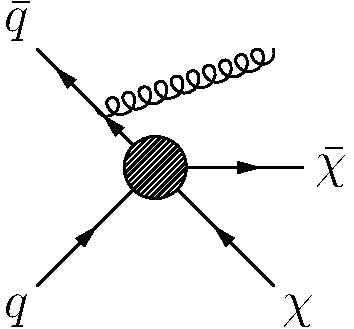
\includegraphics[width=0.2\textwidth]{figs/mono-jet_1}  
\end{center}
\caption[DM production via EFT operator]{\em\label{fig:prod:EFT} Representative diagram for DM pair $(\chi, \bar \chi)$ production 
via a {\bfseries non-renormalizable operator}, represented by a shaded blob. For the process to be observable an initial-state emission of SM particles is needed. 
In the above diagram a gluon is emitted from the initial anti-quark leg, resulting in a mono-jet signature.}
\end{figure}

Keeping all possible operators up to a particular operator dimension then captures the effects of many DM theories.  This approach is systematic in its nature. One simply assumes the spin of DM (usually 0, 1/2 or 1) and writes down
all possible operators up to, let's say, dimension-7 operators involving two DM particles and the SM particles~\cite{NROcolliders}.
An example of a dimension 6 operator is
\beq \label{eq:effop6}
\Lag_{\rm EFT}\supset-\frac{1}{\Lambda^2}(\bar q \gamma_\mu q) J^\mu_{\rm DM},\qquad
J^\mu_{\rm DM} \sim \left\{
\begin{array}{ll}
S^* i\overset{\leftrightarrow}\partial_\mu S & \hbox{if DM is a scalar $S$,}\\
\bar \chi \gamma_\mu \chi & \hbox{if DM is a fermion $\chi$,}\\
\end{array}\right.
\eeq
where $q$ is a quark field: either the left-handed electroweak doublet
$Q = (u,d)_L$ or the right handed weak singlets  $u_R$ or $d_R$. 
The quark flavor indices are omitted. 
The operator is suppressed by the effective new-physics scale $\Lambda$. 
Full electroweak quark multiplets are needed for consistency,
otherwise weak corrections grow with energy. 
Significant couplings to light quarks or gluons
are most important for having a large cross section for DM production at the
$pp$ LHC collider. 

\smallskip

The operators in eq.~\eqref{eq:effop6}  can arise from a tree level exchange of a heavy vector, $V^\mu$, with the interaction Lagrangian $\Lag_{\rm int}\supset \sum_q g_q \big(\bar q \gamma_\mu q) V^\mu +  g_{\rm DM} J_\mu V^\mu$, in which case 
\beq
\label{eq:Lambda:match}
\frac{1}{\Lambda^2}=\frac{g_q g_{\rm DM}}{m^2},
\eeq where $m$ is the mass of the mediator and $g_{q({\rm DM})}$ its coupling to quarks (DM). In deriving this expression the propagator of the mediator  was approximated as $1/(q^2-m^2)\to -1/m^2$, where $q$ is the momentum flowing through the propagator line connecting quarks to DM. This approximation is equivalent to ignoring  dynamics associated with the mediator: the mediator is integrated out, rendering the interaction point-like. All the information about the mediator is still in principle available at low energies, encoded in the form of higher derivative operators (i.e., operators suppressed by powers of $q^2$) and the values of their coefficients, however the expansion is usually truncated to make the problem tractable.
The EFT approximation breaks down when $q\sim m$, i.e., when the energies in the collision are comparable to the mass of the mediator.  

The EFT approach is ideal for describing the results of direct detection experiments, where $q\lesssim 200$ MeV, which is much less than the mediator mass in most DM models, see section \ref{sec:Effective:operators}. 
The use of EFTs to describe the results of LHC searches for DM is more questionable. 
The cross sections induced by non-renormalizable operators tend to grow with energy.
For example, dimension-6 operators like the one in eq.\eq{effop6} give $\sigma \sim E^2/\Lambda^4$  
for the DM production cross section at colliders
and $\sigma \sim M^2/\Lambda^4$ for the DM annihilation cross section.  This energy dependence might suggest that the high energy hadron colliders could set stringent bounds on the EFT operators. 
However, the EFT interpretation faces two problems. 
Firstly, the highly energetic events are less probable, since they require one quark in the proton to carry a large fraction of the proton momentum. The available statistics  is thus smaller, despite the larger cross sections. 
Secondly, the EFT description is valid only for 
\beq E \circa{<}  \min (m, 4\pi \Lambda),
\eeq
where $m$ is the mediator mass.
For energies above $\sim m$ the full theory is needed.
For energies above $\sim 4\pi \Lambda$ the cross section mediated by an
effective operator violates unitarity, signaling a breakdown of the theoretical description.  
This happens when the couplings in the full theory become nonperturbative, typically when $g \sim 4\pi$ is reached.\footnote{
The unitarity bounds computed at tree-level, with all the order one factors included, are generally not more precise than this estimate.
In the large coupling regime the non-perturbative effects become important, and thus the estimates based on perturbation theory  become unreliable.}
Moreover, translating the  bound on $\Lambda$ into a  bound on $m$
requires the knowledge of coupling constants 
$g_q, g_{\rm DM}$, see eq.\eqref{eq:Lambda:match}. 
The largest mass of $m$ the measurement is sensitive to is obtained in the non-perturbative limit, 
$g_{q,{\rm DM}}\sim 4\pi$. 

Typically, the bounds from the LHC searches for DM do not reach the  $\Lambda \gg E$ regime, i.e., the regime for which 
the effective operator description is valid, except for when $g_q, g_{\rm DM}$ are close to the non-perturbative limit. This makes the EFT approach less applicable to the interpretation of the LHC searches.  
Part of the problem can be traced to the fact that the typical DM signals require an emission of 
a visible SM particle either from the initial or the final state, resulting in the mono-jet, mono-photon, mono-$Z$,
mono-higgs, ..., signals. 
Experimentalists need this visible particle to tag the event.  
The price for adding an extra particle is the reduction in the cross section by a factor
$\sim g^2/(4\pi)^2 \sim 10^{-3}$, where $g\sim 1$ is the corresponding SM coupling, i.e., either the strong, the weak or the electro-magnetic coupling.  As discussed above, the colliders have accumulated enough luminosity so that one is able to measure the main high-energy  SM processes,
but not enough to probe the processes with substantially smaller cross sections.
Furthermore, at the LHC the signals of the type `mono-something plus missing energy'  are heavily affected by the SM backgrounds.
Sometimes the EFT regime can be recovered by not considering the highest energy bins in the data, thus achieving that $E \circa{<} \Lambda$, even though the highest energy bins are nominally the ones most sensitive to the higher dimension operators. Not using all the available data is less than ideal.  This situation can be avoided by employing the simplified models, a strategy that we discuss next.  


\subsection{Simplified models}
\index{DM theory!simplified models}\index{Collider!simplified models}
The problem with the effective operators can be rephrased in more physical terms:
the main signal at the hadron colliders is not `DM plus mono-something',
but rather the on-shell production of new particles that mediate interactions between DM and the SM.
Effective operators, introduced as an attempt to avoid dealing with the plethora of possible DM theories, 
do not capture the on-shell production of the mediators and thus miss the most important production channels. 

 It is then better to use a different approach to describe the physics of DM and the mediators at the LHC and build representative cases of DM models --- the `simplified models'. In constructing the simplified models we keep from the complete UV model the smallest number of new physics fields that still describes well the relevant physics: the thermal DM relic abundance and the experimental signatures at the LHC~\cite{SimplifiedDMmodels,DM:simplified:models:reviews}. Simplified models for DM typically have a mediator and the DM field, with different choices for the couplings and the spins of DM and the mediator. The full theory in most cases contains more fields, not just the DM and the mediator. These additional new physics fields are assumed to be much heavier and as such not important for the DM phenomenology.  

\smallskip

Both in the simplified models and in the full models, DM is pair-produced via tree level exchanges of the mediator, either in the $s$- or $t$-channel, or via loop level mediator exchanges, see fig.~\ref{fig:prod:mediator}. 
An example of an $s$-channel mediator is the heavy vector mediator, $V^\mu$, that we introduced in the discussion of EFTs, section~\ref{sec:EFTs?}, eq.~\eqref{eq:Lambda:match}. 
The most commonly considered simplified models are:
\begin{itemize}
\item[$\blacktriangleright$]
{\bf $\mb{s}$-channel color-neutral vector or axial-vector mediator}.
The interaction Lagrangians are (assuming flavor conservation)
\beq
\label{eq:vector:simplified:model}
\Lag_{\hbox{\tiny(axial-)vector}}=-g_{\rm DM}V_\mu J_{\rm DM}^\mu-\sum_f g_f V^\mu \bar f \gamma_\mu (\gamma_5) f,
\eeq
with the DM current $J_{\rm DM}^\mu$ given in \eqref{eq:effop6}. The sum runs over the SM quarks $q=u,d,s,c,b,t$, charged leptons, $e,\mu,\tau$, and neutrinos (for which $f\to P_L\nu$ in \eqref{eq:vector:simplified:model}). To reduce the number of parameters flavor universality is usually assumed, so that the above simplified models depend only 
on a few parameters: 
the mediator mass, $m$, the DM mass, $M$, couplings to quarks, $g_q$, to leptons, $g_\ell$, and to DM, $g_{\rm DM}$, (where $g_q\equiv g_u=g_d=g_s=g_c=g_b=g_t$, and $g_\ell=g_e=g_\mu=g_\tau=g_{\nu_e}=g_{\nu_\mu}=g_{\nu_\tau}$). In the numerical benchmarks the limit $g_{\rm DM}\gg g_{q,\ell}$ is taken, working either in the leptophobic, $g_\ell=0$, or the leptophilic, $g_{\ell}\ne0$, limit. These choices simplify the analysis of data, but still showcase the sensitivities of various LHC searches. In concrete UV models flavor universality may not be realized, so that once DM is discovered the above assumptions can and should be relaxed. 
\item[$\blacktriangleright$]
{\bf $\mb{s}$-channel color-neutral scalar or pseudo-scalar mediator}. 
In this case some care is required in the construction of the simplified models. For instance, considering a simplified model with a pseudo-scalar mediator $a$, the interaction Lagrangian  ($y_f$ are the SM Yukawa couplings)
\beq
\label{eq:Lint:PS}
\Lag_{\hbox{\tiny pseudo-scalar}}=-g_{\rm DM}a \bar \chi i \gamma_5 \chi-\sum_f g_f y_f a \bar f i \gamma_5 f,
\eeq
 does not lead to a theoretically consistent simplified model above the electroweak scale. The interactions in \eqref{eq:Lint:PS} lead to unitarity violating predictions for cross sections since the Lagrangian is not invariant under electroweak gauge transformations (the scalar interactions couple SM fermions of  left- and right-handed chirality, which are in different EW representations). For instance, the amplitudes 
 $\mathscr{A}(q b\to q' ta)\propto \sqrt{s}$ and $\mathscr{A}(gg\to Z a)\propto \ln^2 s$ diverge in the limit of large center-of-mass energy $\sqrt{s}$. 
 To unitarize the two cross sections $a$ needs to be embedded in a full EW multiplet. 
 The additional diagrams from the exchanges of a charged Higgs, $H^\pm$, which would be part of such an EW multiplet, would make the cross section predictions finite. 
 However, the embedding of $a$ into an EW multiplet is not unique. In principle, there are many viable simplified models for $s$-channel color neutral scalar or pseudo-scalar mediators. For a pseudo-scalar mediator the community has endorsed the use of the simplest choice: a two Higgs doublet with a singlet pseudo-scalar that couples to DM (the 2HDM+$a$ model) \cite{DM:simplified:models:reviews}.  However, it is important to remember that this is by far not the only viable possibility and that the details of LHC exclusions depend on the details of the model, such as the relative importance of the mono-jet ($pp\to j+E_T^{\rm miss}$), mono-Higgs ($pp\to H+E_T^{\rm miss}+X$), mono-$Z$ ($pp\to Z+E_T^{\rm miss}+X$), $pp\to t\bar t +E_T^{\rm miss}$, and $pp\to tX+E_T^{\rm miss}$ channels.   

\item[$\blacktriangleright$] {\bf $\mb{t}$-channel color-triplet scalar or pseudo-scalar mediator}. 
If the mediator, $\eta_q$, carries a QCD charge the pair of DM particles  is produced via the $t$-channel exchange of the mediator. The color triplet mediator, see fig.~\ref{fig:prod:mediator} (right), then plays a similar role as do squarks in supersymmetry. However, in the simplified model 
the couplings to quarks are not constrained by supersymmetry, and can be varied freely. 
The interaction Lagrangian is (in Weyl notation)
\beq
\label{eq:Lint:colormed}
\Lag_{\rm triplet}\supset y_q\,  q \chi\eta_q+ \hbox{h.c.},
\eeq
where DM $\chi$ was taken to be fermionic, and the mediator bosonic; 
the other option is also viable.
The EW quantum numbers of $\eta_q$ are the same as the quarks it couples to, i.e., the $\eta_q$ is an EW doublet if it couples to the left-handed SM quarks. A more common choice is that $\eta_q$ is an $\SU(2)_L$ singlet that couples to right-handed SM quarks.  For LHC phenomenology the flavor composition of the couplings to quarks is also important --- common choices are assuming no flavor violation and either flavor universal couplings to the first two generations of quarks or a nonzero coupling to either $b_R$ or $t_R$. 
\end{itemize}
\begin{figure}[!t]
\begin{center}
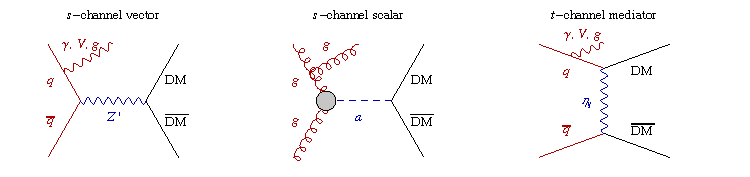
\includegraphics[width=0.95\textwidth]{figs/LHCsearchesFeyn} \vspace{-1ex}
\end{center}
\caption[DM production via mediator]{\em\label{fig:prod:mediator} 
Representative diagrams for the DM production via $s$-channel (axial-)vector mediator (left panel), $s$-channel (pseudo-)scalar mediator (middle), 
and $t$-channel mediator (right). 
}
\end{figure}
There are several important differences between the phenomenology of simplified models and the EFT discussion in section \ref{sec:EFTs?}. The comparison crucially depends on the  size of the mass of the mediator, $m$, relative to the typical momentum exchanged in the collision, $\hat s_{\rm th}$ (the cross sections drop quickly as $1/\hat s^n$, so that they are dominated by the threshold, $\hat s_{\rm th}$). The $\hat s_{\rm th}$ is set by the cuts imposed in the experimental analyses, such as the minimal required $p_T$ of the recoling jet, or the amount of the missing momentum $\slashed E_T$ (momentum carried away by the DM pair).  As a rule of thumb we can take, $\hat s_{\rm th}\simeq 4 M^2+\slashed E_T^2$, with $M$ the DM mass. A typical analysis would vary $\slashed E_T$ between several 100 GeV up to several TeV. 

\smallskip

Focusing on $s$-channel mediator models we can distinguish three regimes: {\em i)} light mediators, $m^2\ll \hat s_{\rm th}$, {\em ii)} the resonant region, $m^2\gtrsim \hat s_{\rm th}$, and {\em iii)} the EFT regime, $m^2\gg \hat s_{\rm th}$. In the light mediator regime, $m^2\ll \hat s$, the mediators are produced off-shell.  The propagator of the mediator can be approximated by $1/(\hat s-m^2)\to 1/\hat s$. This is the exact opposite of the EFT limit, where in the mediator propagator the $\hat s$ can be neglected compared to the heavy mass, $1/(\hat s- m^2)\to -1/m^2$. Using EFT predictions in the regime of light mediators is thus not warranted and leads to erroneous constraints that are too strong (since $1/m^2\gg 1/\hat s_{\rm th}$). 

In the resonant regime, $m^2\gtrsim \hat s_{\rm th}$,  the mediators are produced on-shell. The $pp \to {\rm mediator} \to {\rm DM}\,{\rm DM}$ cross section is enhanced by the resonant production of the mediator to $\sigma(pp\to {\rm mediator}) \sim g_q^2/(4\pi m^2)$, 
compared with the cross section 
$\sigma(pp\to {\rm DM~DM}) \sim g_q^2g_{\rm DM}^2 \hat s_{\rm th} /((4\pi)^3 m^4)$ that is obtained when EFT is assumed to be valid. The EFT prediction for $\sigma(pp\to {\rm DM~DM})$ is kinematically suppressed, as well as suppressed by the relative phase space factor, $1/(4\pi)^2$, 
due to the emission of two DM particles instead of a production of a single mediator.
The cross section calculated using the EFT therefore underestimates the real production cross section. Assuming EFT instead of the on-shell mediator production  thus  leads to over-conservative limits in the resonant region.

  In the narrow-width approximation the resonant production cross section is given by
\beq 
\sigma(pp \to  {\rm DM}\,{\rm DM}) \approx \sigma(pp \to {\rm mediator}) {\rm BR}({\rm mediator}\to  {\rm DM}\,{\rm DM}).
\eeq
The strength of the DM signal in the resonant region therefore depends on the branching ratio for the decay of the mediator to a pair of DM particles. For a mediator that is much heavier than the DM and the SM quarks, we have ${\rm BR}({\rm mediator}\to  {\rm DM}\,{\rm DM})\simeq g_{\rm DM}^2/(g_{\rm DM}^2+ 3 N_f g_q^2)$, assuming that DM is a Dirac fermion, and that only decays to $N_f$ flavors of SM quarks and to DM are open ($g_q$ is taken to be flavor universal for simplicity). For $g_q\gg g_{\rm DM}$ the mediator decays dominantly to SM quarks, while for $g_{\rm DM}\gg g_q$ the mediator decays invisibly to two DM particles. 
Other decay channels can also be open. For instance, the mediator can decay to charged leptons: the $e^+e^-, \mu^+\mu^-, \tau^+\tau^-$ pairs, or have more complicated decay chains. To properly explore the allowed parameter space of the simplified model all these final states need to be taken into account. 

\begin{figure}[!t]
\begin{center}
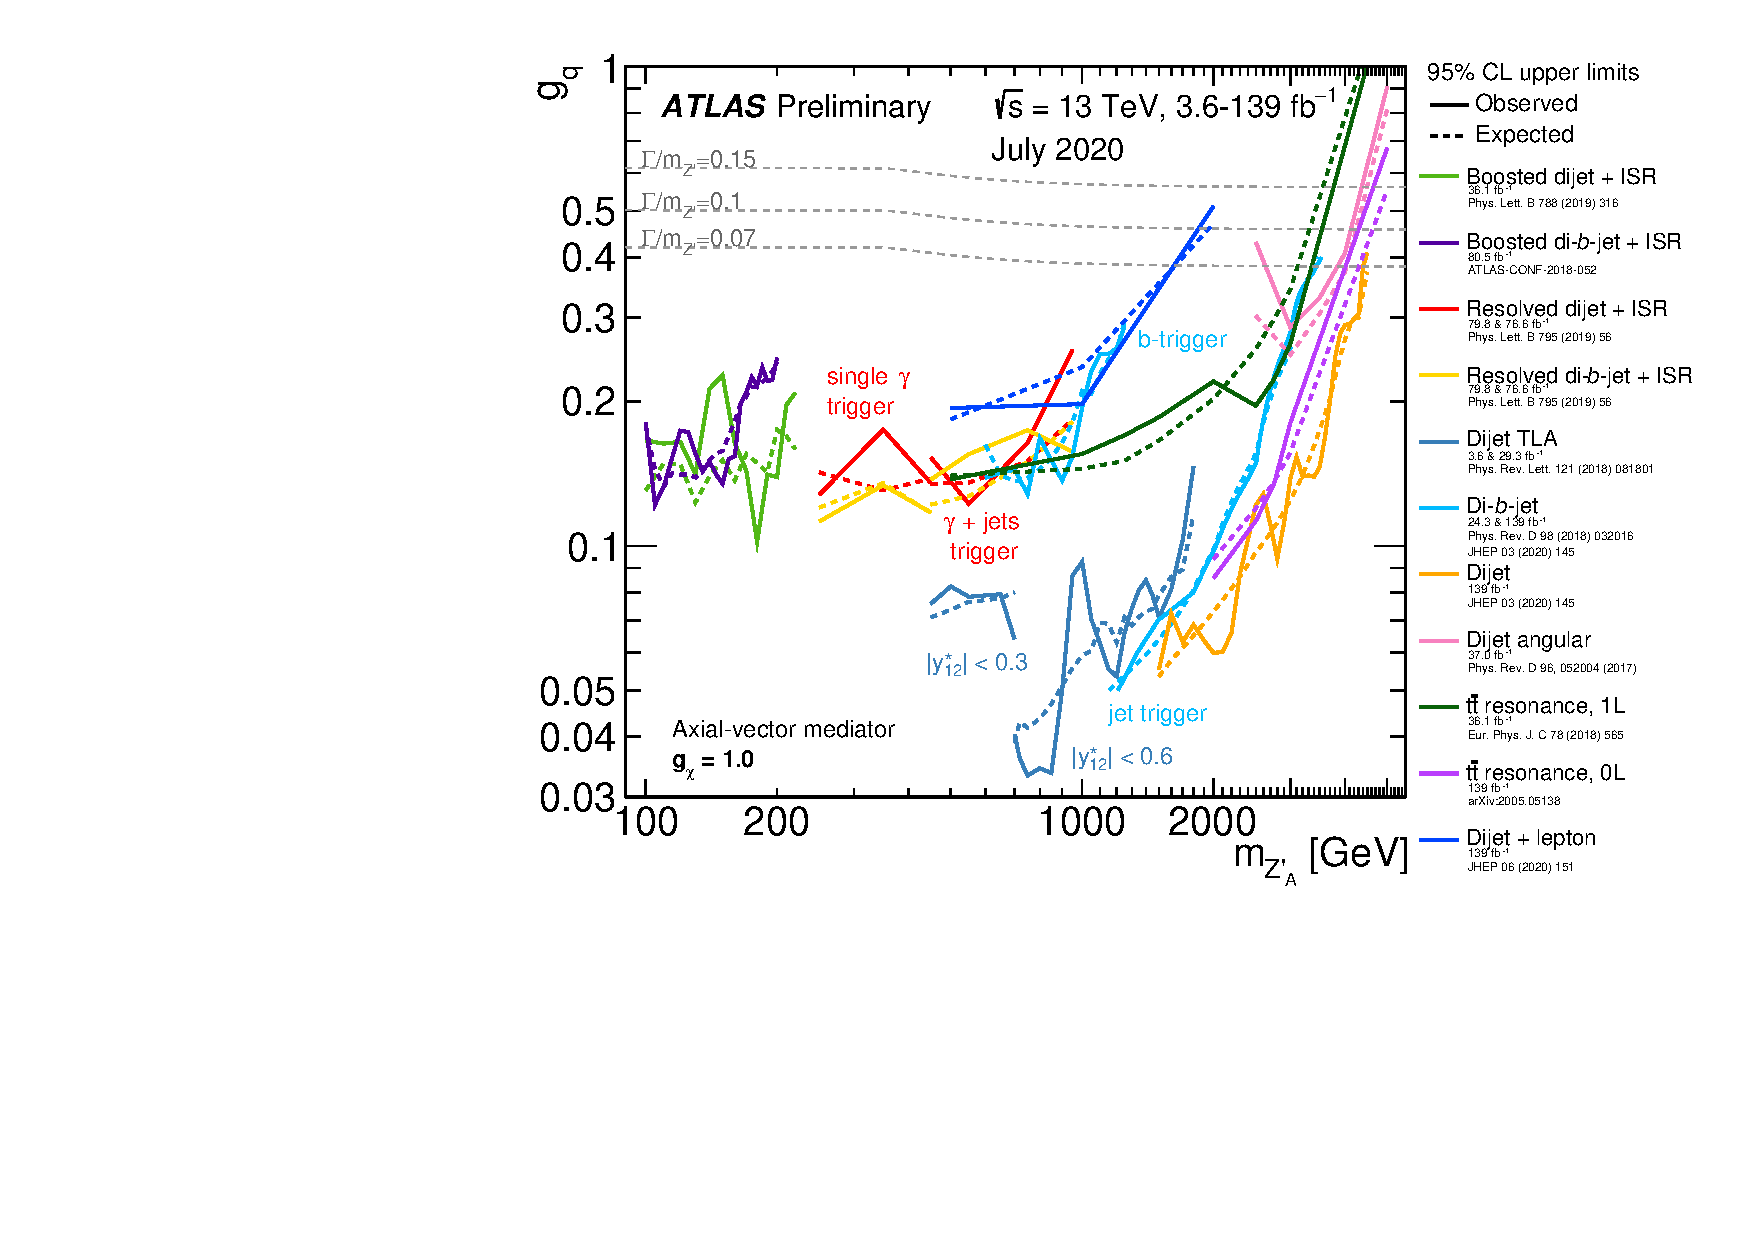
\includegraphics[width=0.7\textwidth]{figs/ATL-PHYS-PUB-2020-021_fig_01} 
\end{center}
\caption[Constraints on vector mediator]{\em\label{fig:vec:mediator} {\bfseries Constraints on axial-vector mediator} $Z_\mu'$, with flavor universal couplings, $\Lag_{\rm int}=g_q\sum_{q=u,d,s,c,b,t} Z_\mu' \bar q \gamma^\mu \gamma_5 q+g_{\rm DM} Z_\mu' \bar \chi \gamma^\mu \chi$ obtained by the ATLAS collaboration from various analyses of $pp$ collisions at the LHC. In the figure the coupling to DM  is fixed to $g_{\rm DM}=1$ (denoted as $g_\chi$ above). Figure from \cite{ATL-PHYS-PUB-2020-021}.}
\end{figure}


\medskip

Finally, for heavy mediators, $m^2\gtrsim \hat s$, the EFT and the simplified model descriptions coincide. The exact point where the EFT description suffices depends on the experimental errors -- for less precise measurements the EFT description can be assumed already for lower  mediator masses. For LHC searches the transition from 
the resonance region to the EFT regime typically occurs for $s$-channel mediator masses $m\gtrsim{\mathcal O}(3~{\rm TeV})$. 

\medskip

As we saw above, the mediator phenomenology depends crucially on the mediator mass $m$.
For instance, the deviations from the effective operator limit are important if $ E\circa{>} m$ and are captured by the simplified models. The other important aspect of simplified models, that is completely missed by the EFT description of DM--SM interactions,  is that the mediators can be searched for using other probes, not only through the decays to DM. The mediators in general couple to quarks, leptons and DM. The coupling to quarks and leptons can then lead to deviations in channels that have in principle nothing to do with DM.  The correlations between such different probes are kept in simplified models, but are not kept in the EFT description. For instance, in EFT the four-quark operators and the quark-quark--DM-DM operators are taken to be completely uncorrelated, while in a simplified $V^\mu$ model the two corresponding  coefficients are given by ${g_q g_{\rm DM}}/{m^2}$ and ${g_q^2}/{m^2}$, see eq.~\eqref{eq:Lambda:match}, and are clearly correlated.

For LHC searches to be relevant, the mediator necessarily couples to quarks and/or gluons. This means that the mediator will also decay to quarks and gluons, and the searches at the LHC such as $pp\to V^\mu \to q\bar q$ also apply. The creation of a quark-antiquark pair appears as two jets in the detector. 
The relevant experimental searches at the LHC are the bump-hunting in the dijet samples of different quark flavors. The exclusions obtained by ATLAS are shown in figure~\ref{fig:vec:mediator} for axial-vector (with the constraints roughly the same for vector mediators $V^\mu$). Since the dijet searches are more constraining than the missing energy searches, 
the null results at the LHC imply $g_q\ll g_{\rm DM}$ for simplified models that are not excluded by the LHC searches (for mediator masses, $m\in[0.1,4]$ TeV, explored by the LHC). 

\medskip

As already stressed above, when constructing  simplified models it is important that the models obey the electroweak gauge symmetry, since the energies involved can be well above the  electroweak symmetry breaking scale.  For instance, a spin 0 mediator $S$ can have Yukawa couplings to pairs of SM fermions 
only if it is appropriately charged under the SM gauge interactions (e.g.,~$S$ can be a Higgs doublet). The other option is that spin-0 mediators have trilinear or quartic couplings to the Higgs, $\Lag_{\rm int}\supset \mu\, SH H^\dagger+ \lambda S SH H^\dagger $, 
and then couple to SM fermions through Higgs-$S$ mixing after Higgs obtains the vacuum expectation value, 
$H= (0,v+h/\sqrt {2})$. In this case $S$ can also be a singlet under the SM gauge group. The models become more complicated for the case of a pseudo-scalar mediator, see the discussion surrounding eq.~\eqref{eq:Lint:PS}.

A particularly interesting possibility for the LHC searches are the $t$-channel mediators $\eta_q$ with squark-like Yukawa
couplings to quarks and DM, eq.~\eqref{eq:Lint:colormed}.
Since the $t$-channel mediators carry color, they can be efficiently pair produced in the $pp$ collisions,  $pp\to \eta_q \eta_q^*$, and searched for through their various decays.

\medskip

In conclusion, simplified models capture the relevant features of full DM models, 
if  a mass gap separates DM and a single mediator from the rest of the spectrum. 
By no means does this exhaust all the possibilities, especially if the full DM theory contains a number of states that are close in mass to the DM. An important example of the latter is DM whose relic abundance is fixed by co-annihilations. In simplified models one still needs to make a number of choices for mediator couplings (for instance, the flavor composition of couplings to quarks, whether or not the mediators couple to leptons, etc). 
While simplified models assume minimal field content, the freedom of choice for various couplings results in simplified models that are not so very simple. 

\medskip

An even more minimal possibility is that the mediator is not a new physics state but rather one of the neutral SM particles, 
such as the Higgs or perhaps the $Z$ boson~\cite{SMmediators}.
A sensitive collider signal arises
if DM is so light that the SM particle can decay into DM, acquiring
an invisible decay width.
Bounds on the invisible Higgs branching ratio, 
$\hbox{BR}_{\rm inv} \circa{<}0.11$ at 95\% C.L., can be obtained either simply
from the Higgs production rate 
(knowing that $\Gamma(X\to h)=\Gamma(h\to X)$, see e.g.~\cite{1303.3570})
or through dedicated searches~\cite{htoinvisibles}. These place severe constraints on the Higgs portal DM, such that DM can be the thermal relic only if it is heavy enough, so that the Higgs cannot decay into it, $M\gtrsim M_h/2$. 


\begin{table}[t]
\begin{center}
\resizebox{\columnwidth}{!}{
\begin{tabular}{lcccccc}
\multicolumn{2}{c}{\bf Interaction}   & \multicolumn{1}{c}{\bf Direct detection}  & \multicolumn{1}{c}{\bf Indirect detection}  & \bf Colliders
\\
Type  & $\Lag_{\rm int}$ &  NR limit, $\chi A \to \chi A$   & $\chi \bar \chi \to q \bar q$ & $\sigma(q\bar q \to \chi \bar \chi)$
\\[1mm] \rowcolor[rgb]{0.95,0.97,0.97}
\hline
 $V\times V$ & $ \big(g_{\rm DM} \bar \chi \gamma^\mu \chi +g_q \bar q \gamma^\mu q \big) V_\mu$  & $1_\chi 1_N$   & $s$-wave & $\sigma_0 $ 
 \\ \rowcolor[rgb]{0.95,0.97,0.97}
  $V\times A$ & $ \big(g_{\rm DM} \bar \chi \gamma^\mu \chi +g_q \bar q \gamma^\mu \gamma_5 q \big) V_\mu$  & $1_\chi (\vec S_N \cdot \vec v_\perp), \vec S_\chi \cdot (\vec q\times \vec S_N)/m_N$   & $s$-wave & $\sigma_0$ 
  \\ \rowcolor[rgb]{0.95,0.97,0.97}
  $A\times V$ & $ \big(g_{\rm DM} \bar \chi \gamma^\mu \gamma_5\chi +g_q \bar q \gamma^\mu q \big) V_\mu$  & $(\vec S_\chi \cdot \vec v_\perp) 1_N, \vec S_\chi \cdot (\vec q\times \vec S_N)/m_N$   & $p$-wave & $\sigma_0$ 
  \\ \rowcolor[rgb]{0.95,0.97,0.97}
    $A\times A$ & $ \big(g_{\rm DM} \bar \chi \gamma^\mu \gamma_5\chi +g_q \bar q \gamma^\mu \gamma_5 q \big) V_\mu$  & $\vec S_\chi \cdot \vec S_N, (\vec S_\chi \cdot \vec q)(\vec S_N\cdot \vec q)/m_\pi^2$   & $p$-wave & $\sigma_0$ 
  \\  
  \hdashline
  \rowcolor[rgb]{0.97,0.97,0.93}
   $S\times S$ & $ \big(g_{\rm DM} \bar \chi \chi +g_q y_q \bar q  q \big) a$  & $1_\chi 1_N$   & $p$-wave & $3 y_q^2 \sigma_0/4$
 \\ \rowcolor[rgb]{0.97,0.97,0.93}
  $S\times P$ & $ \big(g_{\rm DM} \bar \chi \chi +g_q y_q \bar q i \gamma_5 q \big) a$  &   $1_\chi (\vec S_N \cdot \vec q)  m_N/m_\pi^2$ & $p$-wave & $3 y_q^2 \sigma_0/4$
  \\ \rowcolor[rgb]{0.97,0.97,0.93}
  $P\times S$ & $ \big(g_{\rm DM} \bar \chi i \gamma_5 \chi +g_q y_q \bar q  q \big) a$  &  $(\vec S_\chi \cdot \vec q) 1_N /M$   & $s$-wave & $3 y_q^2 \sigma_0/4$
  \\ \rowcolor[rgb]{0.97,0.97,0.93}
    $P\times P$ & $ \big(g_{\rm DM} \bar \chi i \gamma_5\chi +g_q y_q \bar q i \gamma_5 q \big) a$  & $ (\vec S_\chi \cdot \vec q)(\vec S_N\cdot \vec q)m_N/ M m_\pi^2$  & $s$-wave &$3 y_q^2 \sigma_0/4$
\end{tabular}
}
\end{center}
\vspace{-1ex}
\caption[Comparisons of DM production and annihilation cross sections]{\em\label{tab:different:DMint} {\bfseries Comparison of different DM probes} assuming 
as mediators a vector $V_\mu$ or scalar $a$,
and as DM a Dirac fermion $\chi$ with mass $M$.
The first two columns describe the possible chiral structures of couplings to DM and SM quarks $q$, where
$y_q$ is the SM Yukawa; for notation see eq.s~\eqref{eq:vector:simplified:model}, \eqref{eq:Lint:PS}.
The third column lists the leading non-relativistic operators giving rise to DM scattering on nuclei. 
The fourth column indicates whether the $\chi\bar \chi \to q\bar q$ annihilation proceeds through $s$-wave or $p$-wave. 
The last column gives the total cross section for $q\bar q \to \bar \chi \chi$ in the limit where the center of mass energy, $\sqrt s$, is much larger than the DM mass, but still much smaller than the mediator mass. 
The partonic cross section $\sigma_0=g_{\rm DM}^2 g_q^2 (s/m_{\rm med}^2)^2 /(6\pi s)$ needs to be convoluted with the parton distribution functions in order to obtain the $pp\to \chi \chi$ cross section, relevant for the LHC.
}
\end{table}


\section{Comparing collider with direct and indirect signals}
\label{sec:complementarities}
Typically,  DM models lead to potential signals in many of the searches: both in direct detection, indirect detection and collider experiments (the latter in appreciable numbers only if the mediators couple to quarks and gluons). The question thus naturally arises of how to compare the possible signals. 

Simplified models can be used to gauge the sensitivities of different experiments for sample DM models. As can be seen from table~\ref{tab:different:DMint} the strength of the signal can vary widely, depending on the detailed structure of the mediator couplings. In particular, for direct detection and indirect detection the chiral structure of the DM and SM currents is very important. This is a consequence of the non-relativistic nature of DM in the initial state in both direct and indirect detection. Since the axial and vector (similarly, scalar and pseudo-scalar) currents have drastically different non-relativistic limits, this translates into very different expected signals. In table~\ref{tab:different:DMint} we list a few illustrative examples: the four chiral structures of currents for either vector or scalar mediators. The expected sizes of direct and indirect detection signals for many other DM/SM couplings can be found in~\cite{1305.1611}.

\smallskip

The third column in table~\ref{tab:different:DMint}  lists the leading DM/nucleon non-relativistic operators that describe the scattering in direct detection experiments. These operators still need to be sandwiched inside nuclear wave functions to obtain the rate for DM scattering on nucleus (for details see section \ref{sec:DMscatt:nuclei}). However, already at the level of DM/nucleon interactions, and ignoring the complications introduced by the nuclear physics, it is clear that taking the non-relativistic limit leads to drastically different kinematical suppressions for various chiral structures. For instance, the $V\times V$ and $S\times S$ interactions give rise to the numbering operators in the non-relativistic limit (the  operator $1_\chi$ in table~\ref{tab:different:DMint}  counts the number of DM particles, while $1_N$ counts the number of nucleons).  Consequently, the spin-independent DM/nucleus scattering is coherently enhanced, schematically $\sigma \propto A^2$, where $A$ is the mass number of the nucleus, since the nuclear matrix element is proportional to the number of neutrons and protons in the nucleus.
Such enhancement is not present for the other chiral structures. The $A\times A$ interaction leads to spin-dependent scattering (in table~\ref{tab:different:DMint} $\vec S_\chi$ denotes the DM spin, $\vec S_N$ the nucleon spin), while the remaining chiral structures are even further kinematically suppressed by either the momentum exchange, $\vec q$, or by the initial relative velocity between DM and the nucleon, $\vec v_\perp$ (a scaling discussion of relative sizes of different contributions can be found in \cite{1809.03506}). 

\smallskip

In indirect detection only the DM is non-relativistic, while the outgoing quarks are highly relativistic (we assume $M \gg m_q$). The relative angular momentum between $\chi$ and $\bar \chi$ determines the velocity suppression of the $\bar \chi \chi \to q\bar q$ annihilation  cross section, $\sigma v_{\rm rel}=\sigma_L v_{\rm rel}^{2L}$, see also the discussion below eq.~\eqref{eq:gamma:ann}. That is, the $L=0$ ($s$-wave) annihilation is not velocity suppressed, while $L=1$ ($p$-wave) annihilation is.  The transformations of the DM bilinear under rotations, combined with $C$ and $P$ transformations, fully determine the total angular momentum, the spin and the orbital angular momentum of the initial state that this bilinear annihilates, and thus whether the $s$-wave annihilation is possible. We see that the pattern of suppressed and unsuppressed signals is quite different from the one in direct detection. For instance, while in direct detection both $V\times V$ and $S\times S$ interactions lead to coherently enhanced DM/nucleus scattering, in indirect detection the $S\times S$ interactions leads to velocity suppressed $p$-wave annihilation, in contrast to $V\times V$, which gives rise to the unsuppressed $s$-wave annihilation. Similarly, while $V\times A$, $P\times S$, and $P\times P$ lead to suppressed direct detection signals, they give rise to unsuppressed $s$-wave annihilation signals in indirect detection. 

\smallskip

The final column in table~\ref{tab:different:DMint} gives the expected sizes of the DM pair production cross sections at colliders such as the LHC. Instead of discussing the production cross sections for the monojet signal, 
$pp\to \chi \bar \chi +\,$jet, we use as a proxy the size of the simpler $q\bar q\to \chi \bar \chi$ scattering cross section. Even so, the conclusions we draw apply more generally. For simplicity we work in the limit of heavy mediators and with the energy of the collision much greater than the DM mass. Unlike the direct and indirect detection, for collider physics the chiral structure of the interactions has little effect on the size of the production cross sections. This is easy to understand from naive dimensional analysis, since the only scale in the problem is  the collision energy, $\sqrt s$. The structure of the interaction only tells us whether just left-handed or right-handed or both chiralities participate in the interaction, which changes the predictions for the cross section by factors of 2. In the examples in table~\ref{tab:different:DMint} the cross sections for the vector mediator (and separately for the scalar mediator) do not even differ by such factors of 2, and are instead the same for all chirality structures, a consequence of the fact that  the interactions have definite transformation properties under parity.

\smallskip

In conclusion, the observation of a signal in one set of experiments and non-observation in another could pinpoint  to the nature of DM interactions with the SM. 


\section{Searches with beam dumps and precision measurements}\index{Beam dump}
\label{sec:searches:beam:dumps}
Dark matter could be part of a more complicated dark sector. This has significant consequences for experimental searches.
Instead of just searching  for the DM particle, a more general search strategy tries to produce any of the 
(possibly lighter) particles in the dark sector.  
The discovery of such mediators between visible and dark sector may then give access to the DM itself as well. 
In such `fishing expeditions' the theoretical bias is best kept to a minimum. 
However, completely ignoring theoretical inputs would leave us with a  gigantic space of possibilities. 
A more useful approach is to, at least initially, focus on interactions with the lowest dimension, 
the so called {\it portals}. Keeping only renormalizable operators and operators suppressed by a single power of the high scale gives four distinct possibilities for the mediators:
\begin{itemize}
\item[$\circ$] 
{\bf a light scalar,} usually dubbed either a  {\em``dark Higgs''} or a {\em``light singlet''}, that mixes with the SM Higgs through the portal interaction;
\item[$\circ$] {\bf a light pseudo-scalar}, usually called {\em ``axion''},  with derivative couplings to the SM fermion currents, suppressed by a high scale $f_a$;
\item[$\circ$] {\bf a spin 1/2 fermion}, dubbed {\em ``heavy neutral lepton''} or  {\em ``sterile neutrino''} $\nu_{\rm s}$, 
that couples to the SM leptons and the Higgs via a Yukawa interaction; 
\item[$\circ$] {\bf a spin 1 vector boson}, dubbed {\em ``dark photon''} or  {\em ``light $Z'$''} and denoted as $A'$,  that couples to the SM via kinetic mixing.\index{Dark photon}
\end{itemize}
The theoretical aspects of dark sector portals are discussed in more detail in section~\ref{sec:darksectors}, with a summary given in table~\ref{tab:portals}. 
Here, we mostly concentrate on  the experimental searches for the dark sector mediators, at accelerators or more generally in laboratory set-ups. 

The mediators to dark sectors, listed in table \ref{tab:portals}, can be produced directly in the laboratory experiments, or observed indirectly through effects due to virtual exchanges of the mediators. The phenomenology depends crucially on the mass of the mediator, and falls roughly in one of the three regimes. 
For mediators lighter than an eV, the Compton wavelength is of atomic size or larger, all the way to macroscopic or astrophysical sizes. 
For masses in the MeV to TeV range the mediators can be produced in typical particle physics experiments. 
Heavier mediators, in contrast, can only be observed through their off-shell exchanges.
Light particles are subject to strong bounds that forbid electric, weak and strong charges,
in agreement with DM properties.

\begin{figure}[!t]
\begin{center}
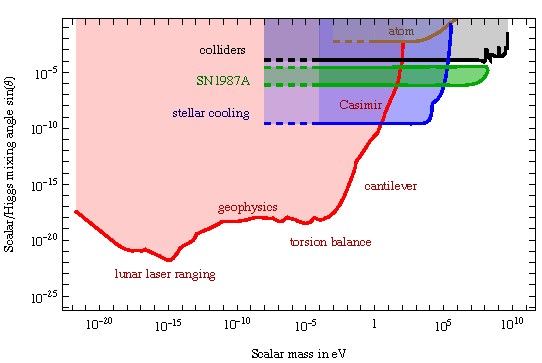
\includegraphics[width=0.68\textwidth]{figs/Fig_Higgs_Scalar} 
\end{center}
\caption[Constraints on Higgs mixed scalar]{\em \small \label{fig:Higgs:mixed:scalar} 
{\bfseries Constraints on a light scalar that mixes with the Higgs} as a function of the mixing angle $\theta$ for a wide range of scalar masses \cite{Portals,fifth:force:reviews,AMO:dark:sector,isotopic:shift,stellar:cooling,SN:constraints}. In the constraints we assumed that the coupling to DM is subdominant to the Higgs-induced couplings to the SM fermions.
If the coupling to DM is important, this would affect only the high-mass boundaries of the collider (black), supernova (green) and stellar cooling (blue) exclusions. There are further constraints from colliders for scalar masses in the $100\GeV$ to $\TeV$ range, which are not shown, since they are model dependent (they do not depend just on the mixing angle).
}
\end{figure}



\subsection{Mediators with sub-eV masses}
\label{sec:mediators-sub-eV}
Very light mediators, with sub-eV masses, generate new macroscopic forces. A tree level exchange of a light $Z'$ vector mediator or a light scalar of mass $m_{\rm med}$ generates a potential between two particles of the form
\beq
\label{eq:Vpot}
V_{ij}(r)=- \alpha_{ij} \frac{e^{-m_{\rm med} r}}{r}.
\eeq
The coupling constant is $\alpha_{ij}=+ g_{i} g_{j}/4\pi$ for the scalar mediator, and $\alpha_{ij}=- g_{i} g_{j}/4\pi$  for the vector mediator, where $g_i$ is the coupling constant for interaction between the mediator and the $i$-th particle.  This means that the potential between two particles of the same specie
--- for instance, between two protons or two electrons --- is always attractive (repulsive) for the scalar (vector) mediator. For particles of different species, e.g., between a proton and an electron, the potential can be of either sign. Furthermore, the form of the potential in eq.~\eqref{eq:Vpot} is not the only possibility: for instance, a pseudo-scalar mediator or a mediator that couples to the SM fermions through higher dimension operators would  induce spin-dependent potentials, see, e.g.,~\cite{spin:dependent:forces}.

The range of the potential is controlled by the mass of the mediator, and is given by
\beq
\lambda \equiv \frac{1}{m_{\rm med}}=\, 197\,{\rm nm}\, \frac{{\rm eV}}{m_{\rm med}}=0.2\,{\rm m}\,\frac{{\rm \mu eV}}{m_{\rm med}}=1.3\,{\rm a.u.}\frac{10^{-18}{\rm eV}}{m_{\rm med}}=0.6\, {\rm kpc} \frac{10^{-26}{\rm eV}}{m_{\rm med}},
\eeq
where we chose numerical examples for the mediator mass that correspond to atomic, macroscopic, solar system and galactic sizes, respectively. 
In view of such disparate scales there are a number of very different experimental searches for mediator-induced long range potentials. 
Many of these searches share a strong similarity with those discussed in section \ref{AxionExp} for axion DM. 


\subsubsection{Fifth force experiments} \index{Fifth force}
Fifth force experiments measure the gravitational force between two objects using laboratory setups. They search for deviations from the $1/r^2$ dependence by comparing the force at two or more distances \cite{fifth:force:reviews}. The limits on the strength of non-gravitational interactions is given in terms of $\alpha\equiv \alpha_{ij}  G/m_i m_j$, where $G$ is the Newton constant, and $m_{i,j}$ are the masses of the two test objects. That is, for $r\ll \lambda$ the constant $\alpha$ gives the strength of the ``fifth force'' relative to the force of gravity. The strongest constraints are obtained for $100\,{\rm \mu m }\lesssim \lambda \lesssim 10\,{\rm m}$ using torsion balances, giving $\alpha \lesssim 10^{-3}$. For $\lambda\simeq 10 \,{\rm \mu m }$ to $\sim 100\,{\rm \mu m}$  the cantilevers are used as force sensors instead of torsion balances, while for even smaller distances, up to $0.1\,{\rm \mu m}$, the experiments measuring the Casimir forces are used. Since at such distances the electromagnetic interactions become important, the sensitivity quickly deteriorates all the way up to $\alpha \sim 10^{30}$. At larger distances the constraints come from the tests of Keplerian motion and have decent sensitivity up to $\lambda\gtrsim 10^{14}$ m. The  best sensitivity is reached at scales $\lambda\approx 10^{8}$\,m, where the bounds from lunar laser ranging give $\alpha \lesssim 10^{-10}$. 

\subsubsection{Tests of the weak equivalence principle}
It the coupling constant $\alpha_{ij}$ in eq.~\eqref{eq:Vpot} is not proportional to the product of test masses, $m_i m_j$, then the force induced by the light mediator violates the weak equivalence principle as it depends not just on the total mass of the probe but also on the type of the material used in the  experiment \cite{fifth:force:reviews}. 
Tests of the weak equivalence principle are in general more sensitive than the tests of the $1/r^2$ dependence. They probe scales from cm to a.u., where the precise sensitivity dependends on the relative sizes of the couplings $g_i$ for different SM fundamental particles (the couplings to $u$ and $d$ quarks, to gluons, and to electrons).


\subsubsection{Atomic transitions} \index{Atomic transitions}
At smaller distances,  comparable to the size of an atom, the dominant SM force is the electromagnetic interaction. 
The presence of portal mediators with   $\lambda\sim {\mathcal O}(100\, {\rm nm})$ would correct the $1/r$ electrostatic potential between the electrons and the atomic nucleus, changing the atomic levels away from the SM predictions. 
The experimental precision on these is stunning, with the fractional frequency precision of atomic frequency standards based on microwave and optical transitions reaching the levels $\delta \nu /\nu\sim 10^{-16}$ and $\delta \nu/\nu \sim 10^{-18}$, respectively \cite{AMO:dark:sector}.  The main problem in converting the experimental measurement to bounds on new physics particles is that the precision of the SM theoretical predictions are nowhere near the above precision. One can bypass this problem, at least to some extent, by taking advantage of the special features of the new physics signal. 

For instance, if the dark mediator has couplings that are not just the rescaled electric charges, then one can use the measurements of atomic transitions for several different isotopes to cancel out the leading electromagnetic effects. In this way one can place nontrivial bounds on the new physics contributions to the electron--nucleus potential \cite{isotopic:shift}.

Another interesting possibility opens up, if either the dark Higgs or the axion constitute part or the majority of the DM relic density. The occupation number per quantum state is large, $N\gg 1$, see section~\ref{LightBosonDM}.
Such background fields therefore behave as classical fields that oscillate coherently with the frequency equal to the mass of the mediator, $m_{\rm med}$, and induce a time dependent change in the potential between electrons and the nucleus. As a result the atomic energy levels become time dependent, a feature that can be searched for. The results are usually {presented} as bound on time dependence of the fundamental constants ($\alpha_{\rm QED}$, quark masses, etc.).
One can also search for spatial variations in the fundamental constants, which would be induced by the spatial variations in the background dark Higgs or axion fields. 


\subsubsection{Stellar cooling} \index{Stars!cooling}
Light dark sector particles can be copiously produced in the stars, thus modifying the stellar dynamics~\cite{stellar:cooling}. An outgoing flux of dark sector particles would carry away energy, possibly leading to excessive cooling. This leads to stringent constraints on the intermediate range of dark sector couplings to the visible matter: the couplings large enough such that the dark sector particles are still copiously produced in the stars, but small enough so that the dark sector particles escape from the star and are not trapped in its interior, are excluded. For dark sector particles to be produced the temperature inside the star needs to be high enough, i.e., the temperature needs to be comparable to the particle's mass.
White dwarf cooling thus constrains  dark sector particles with masses below a few keV, red giant cooling constrains masses below several tens of keV, and SN1987A observations below about 100 MeV. 


The stellar cooling constraints are inherently uncertain, since they rely on our understanding of astrophysics. This is especially true for the bounds from SN1987A that rely on the observation of a single supernova event \cite{SN:constraints}. The exotic cooling would shorten the neutrino signal that was observed coincident with the supernova discovery in optical light, but only if the event was due to the standard core collapse supernova \cite{1907.05020}.



\subsubsection{Axion searches} 
Many laboratory experiments are searching for axions. Most of these are explicitly designed to search for the specific coupling of axion to photons, $a F\tilde F$, and are reviewed in section \ref{AxionExp}. 

\subsubsection{Light shining through wall} 
\index{Light shining through wall}
Light shining through wall searches can be used to search for axions (see section \ref{AxionExp}) and for dark photons. 
Dark sector particles are created in the first part of the laser beam, before it hits the wall. The dark sector particles are the only ones that can pass through the wall, and are then converted back into a visible signal behind the wall. A version of this concept is the {\sc DarkSRF} experiment, which used superconducting radio frequency cavities both for creation of dark photons (in the first cavity) and the conversion (in a different, shielded cavity) and achieved best sensitivity, below fifth force searches, for dark photon masses around $\mu$eV, excluding mixing angles larger than $\epsilon\gtrsim 10^{-8}$~\cite{Romanenko:2023irv} (see also results from the {\sc SHANHE} experiment \cite{SHANHE}). 


\subsubsection{Virtual corrections} 
Some observables have been precisely measured, such as the magnetic moments of the electron and the muon, $(g-2)_e$ and $(g-2)_\mu$.
Others are very small in the SM, such as the electric dipole moment of a neutron (nEDM). 
These could be affected by quantum corrections from DM running in the loop \cite{Virtual:DM:contrib}.\footnote{See he discussion of $(g-2)_\mu$ experimental anomaly and possible connection to DM in section \ref{sec:g-2}, and the $m_W$ anomaly in section \ref{sec:CDFWmass}.} 
While the relevance of these constraints depends on the model (for instance, nEDM requires CP violating couplings of DM), they can, in parts of the parameter space,  be more stringent than the more direct searches for DM. Note that the constraints from virtual corrections are relevant both for light DM as well as for heavy DM, with mass in the TeV regime, since DM does not need to be produced on-shell. 


\subsubsection{Neutrino oscillations to sterile neutrinos}\index{Sterile neutrino}
 Light fermions, with masses below ${\rm eV}$, that are not charged under the standard model group are conventionally called sterile neutrinos, $\nu_{\rm s}$. 
 They can have the Yukawa interaction, $\Lag \supset y_{\rm s} \nu_{\rm s} L H  $, with the SM neutrinos, which are part of the weak doublets $L$ (we are suppressing flavor indices).
 After electroweak symmetry breaking the Yukawa interaction, setting the Higgs field to its vacuum expectation value, $\med{H} = (0,v)$, 
 becomes a mass term, $ y_{\rm s}v\, \bar \nu_{\rm s} \nu_L$,
 that mixes sterile and active neutrinos.  Such small mass mixings can be searched for in neutrino oscillation experiments, similarly to how the SM neutrino masses themselves were discovered~\cite{sterile:neutrino:osc}. The interest in light sterile neutrinos has been motivated for the past two decades by a number of experimental anomalies: the LSND and MiniBooNE anomalies, the reactor anti-neutrino anomaly, and in experiments with intense radioactive sources \cite{neutrino:anomalies}. However, none of these  anomalies seems  very plausible at present.


\subsection{Mediators with MeV or GeV masses}\label{sec:collider:lightmediators}\index{Mediators}\index{Collider!light mediators}
This is the typical mass range where particle physics experiments can probe on-shell production of the mediators.  The specifics of each search depends on the production mechanism (such as which particles are being used in the collisions) as well as on the decay products. Figure \ref{fig:dark:photon:constraints} provides a summary of the current constraints.

\begin{figure}[t]
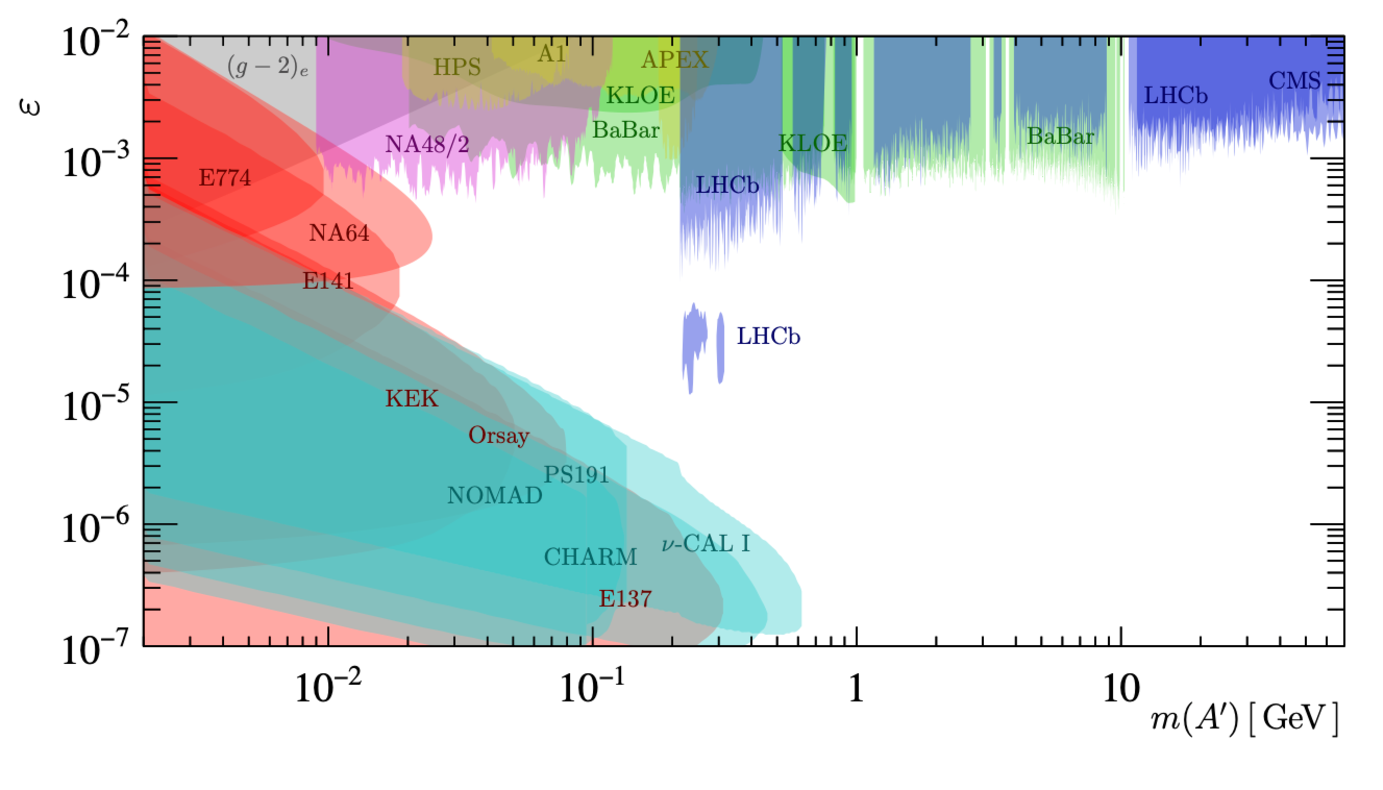
\includegraphics[width=0.47\textwidth]{figs/dark_photon_constraints}
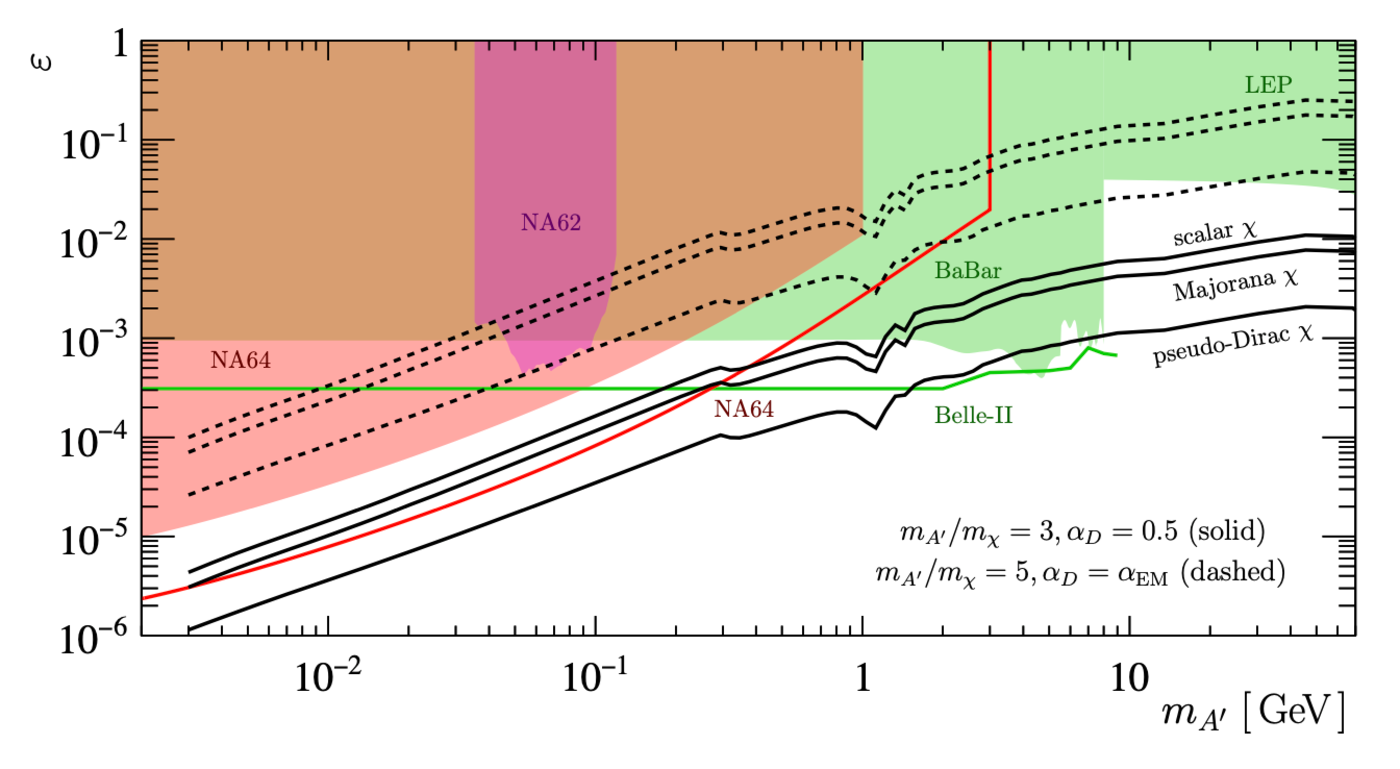
\includegraphics[width=0.49\textwidth]{figs/dark_photon_constraints_inv}
\caption[Dark Photon Constraints]{\em  {\bfseries Left}: Constraints on a vector boson mediator (usually termed a {\bfseries dark photon}, or, sometimes, a light $Z^\prime$) in the plane of the kinetic mixing parameter $\epsilon$ (which controls the strength of interactions with the SM, see section \ref{sec:VectorPortal}) and of its mass, $M_{A'}$, assuming only the visible decays are allowed. 
The constrains are from electron beam dumps (dark red region), proton beam dumps (dark green), $e^+e^-$ colliders (light green), $pp$ collisions (blue), meson decays (magenta), $(g-2)_e$ (grey), and electron on fixed target experiments (yellow). 
The triangular shape of the beam dump constraints is due to the fact that the $A'$ decay length scales as $1/\epsilon^2M_{A'}$. When the $A'$ mass or the mixing $\epsilon$ are too large, the vector boson decays too fast and does not reach the detector.
The collider constraints in the upper part of the plot are instead essentially flat in $M_{A'}$. These searches scan for a new resonant bump in the invariant mass distribution of two SM particles, which would indicate the presence of $A' \to$ SM SM decays. 
{\bfseries Right}: sensitivity to a vector boson mediator (dark photon) that decays invisibly. The solid and dashed black lines denote several DM benchmarks for which the correct thermal relic abundance is obtained.  Both figures are from Graham et al.~in \cite{Dark:photon}.
 \label{fig:dark:photon:constraints} }
\end{figure}


\subsubsection{Searches in $e^+e^-$ colliders} 
A major benefit of the $e^+e^-$ colliders is that the events are clean, with relatively little background activity in the detector \cite{dark:sector:e+e-}. 
The detectors typically cover almost the complete $4\pi$ solid angle around the interaction point, apart from the small region very close to the beam pipe,  which cannot be instrumented.  The visible final states can therefore be fully reconstructed. This in turn means  that  the direction of the missing momentum and/or missing energy, due to the dark sector particles escaping the detector, can be determined precisely. The high-luminosity $e^+e^-$ colliders are primarily used for measurements of rare process with heavy quarks and are thus not very energetic. For instance, the $B$ factories ({\sc BaBar} in the USA and {\sc Belle} in Japan in 2000s), and the upcoming super-$B$ factory {\sc Belle II} in Japan, have the $e^+e^-$ collision energy tuned to the resonant production of the $B\bar B$ meson pairs which occurs close to the production threshold $\sqrt{s}\approx {\mathcal O}(10{\rm~GeV})$. Only mediators lighter than the collision energy can be probed through on-shell production, limiting the dark sector mass reach of such experiments. More massive mediators were probed at LEP, $\sqrt{s}\approx 200$ GeV (in the future at proposed {\sc Fcc} at CERN or {\sc CepC} in China). The mediators can be either produced directly in the $e^+e^-$ collisions, such as $e^+e^-\to A'\gamma$, or from decays of other particles, for instance $e^+e^-\to \tau^+(\tau^-\to \nu_{\rm s} \mu^-\bar \nu_\mu)$. The mediators can either: {\em i)} decay immediately (prompt decays),  {\em ii)} decay away from the interaction point but still in the detector, leading to displaced vertices, or {\em iii)} completely escape the detector leading to missing energy signature. The searches need to be optimized for each of these possibilities, as well as for the choice of the final state. 


\subsubsection{Searches in hadron colliders} 
These searches use the $pp$ collisions at the LHC, which lead to complicated final states with many pions, and other hadronic states produced in a typical collision~\cite{dark:sector:LHC}. Due to the messy hadronic environment the searches for dark sector particles at the LHC are challenging. 
A mitigating strategy is to look for final states and observables that are easily distinguishable, such as the resonant peak  in the $\mu^+\mu^-$ and $e^+e^-$ invariant mass spectra due to  $A'\to \mu^+\mu^-$ or $A'\to e^+e^-$ decays (such searches were performed or are being planned by the LHCb, CMS and ATLAS experiments). The other option is to search for mediators that are produced in the $pp$ collision, but decay far away from the collision point. The backgrounds are reduced to essentially zero by placing the detector behind a shield made of meters of iron, concrete or dirt such that the electromagnetically and strongly interacting SM particles get stopped, while dark sector particles penetrate unobstructed through the shield.  Experiments of this type are {\sc Faser}, and the planned experiments {\sc Codex-b} and {\sc Mathusla}, each to be positioned close to a different collision point in the LHC ring. 

\subsubsection{Searches in electron beam fixed target experiments} 
In these types of experiments a high intensity electron beam is sent on a thin target (or a collection of such targets, most often made of high-$Z$ materials). The electrons in the beam can then produce dark photons or ALPs in the field of the nucleus in the target, while their decays are measured in detectors placed down-stream from the target.\index{Axion-like particles} The benefit over $e^+e^-$ collisions is the potential for very high delivered luminosity, however,
due to the kinematics of a collision with a particle at rest the center of mass energy is lower, and therefore
 the reach in the mediator mass is typically lower than in the $e^+e^-$ collisions or at the hadron colliders. 
 Experiments of this type are A1 (Mainz Microtron), {\sc Apex} (JLAB), {\sc Hps} (JLAB), and NA64 (CERN) \cite{electron:beam:fixed:target}.

\subsubsection{Searches in electron and proton beam dump experiments}  
In these types of experiments a high intensity electron or proton beam is sent on a thick target. The main difference with the fixed target experiments is that the beam dump experiments have detectors behind substantial shielding that absorbs the SM particles. Such experiments are thus not sensitive to prompt decays of mediators, but only to mediators with lifetimes long enough to decay in the detector far from the beam dump target. 
There are a number of proposed beam dump experiments with significantly improved projected reach, including {\sc SHiP} 
and {\sc Shadows} at CERN, and {\sc Pip2-BD} at Fermilab \cite{beam:dump}. 


\subsubsection{Searches in meson and lepton decays} 
Another possible search strategy, with some overlap with the previous ones, is to search for rare decays of mesons ($\pi^0, \eta, K^+, B^0,\ldots$) or leptons ($\tau, \mu$) into dark sector + SM particles, but with the final state fully reconstructed \cite{meson:decays}. The benefit is that this reduces possible backgrounds. In addition, weakly decaying SM particles much lighter than the weak scale have small SM decay rates, 
$\Gamma_{\rm SM}\sim  m^5/M_W^4$ with $m\ll M_W$. This is beneficial when searching for new physics via rare decays, 
since the branching fraction for the rare process gets relatively enhanced by the small total decay width, $\hbox{BR}_{\rm rare}=\Gamma_{\rm rare}/\Gamma_{\rm SM}$.


\subsection{Very heavy mediators, TeV masses or above}\index{Collider!heavy mediators}
Heavy mediators, with masses above a few TeV cannot be produced on-shell in the laboratory experiments since their mass exceeds the collision energy. Nevertheless, we can still search for them indirectly, through their virtual corrections. In order to increase the sensitivity to new physics it is advantageous to choose processes that are extremely rare in the SM, can be well predicted theoretically, and at the same time can receive large contributions from virtual exchanges of the mediators. 

\subsubsection{Flavor-changing neutral current processes} 
Flavor-changing neutral currents (FCNCs), such as $\bar b s\leftrightarrow  \bar s b$ or $\bar s d \leftrightarrow \bar d s$, do not occur in the SM at tree level since the neutral gauge bosons (the $Z$ boson, the gluons and the photon) 
only have flavor-diagonal interactions \cite{Introduction:flavor:physics}. 
The FCNCs first occur in the SM at one loop from $W$ exchanges in the loop, and are suppressed by the loop factor and the products of CKM matrix elements and quark masses. This additional suppression is a manifestation of the ``GIM mechanism'' --- if all the quark masses were the same there would be no flavor violation.


The mediators can have flavor-violating couplings, in which case already the tree level exchanges of mediators induce FCNCs. 
Taking the corresponding flavor-violating couplings to be ${\mathcal O}(1)$, and to have ${\mathcal O}(1)$ CP-violating phases,
the comparison of $K \leftrightarrow \bar K$
(i.e.\  $\bar s  d\leftrightarrow \bar d s$ at quark level),
$D\leftrightarrow\bar D $ ($\bar u  c\leftrightarrow \bar c u$), 
$B\leftrightarrow\bar B $ ($\bar b  d\leftrightarrow \bar d b$) and 
$B_s\leftrightarrow\bar B_s $ ($\bar b s  \leftrightarrow \bar s b$)
mixing rates with the SM predictions bounds vector mediators to have masses $m \gtrsim 2 \cdot 10^{4}\, {\rm~TeV}, 10^4\,{\rm~TeV},10^3\,{\rm~TeV}, 400\,{\rm~TeV}$, respectively \cite{FCNC:bounds}.
These bounds scale as $m/g_{qq'}$, and thus crucially depend  on the size of the flavor violating coupling, $g_{qq'}$, that induces the $q\to q'$ transition. If $g_{qq'}$ is small, the bounds on the mediator mass $m$ become weaker: if the suppression is of the same form as in the SM, i.e., a product of CKM matrix elements and a loop factor, then mediators with weak scale masses are still allowed; if the couplings are even further suppressed, the mediators can be correspondingly lighter. Even more stringent bounds follow from the absence of FCNCs in the lepton sector, for instance, from the bounds on ${\rm BR}(\mu \to e \gamma), {\rm BR}(\tau\to 3\mu)$, etc~\cite{FCNC:bounds}.

\subsubsection{Electric and magnetic dipole moments} \index{Dipole moments}
The FCNC observables are not the only precision observables that give stringent bounds on potential off-shell contributions from the mediators. For instance,  electric dipole moments (EDM) are CP violating but flavor diagonal, i.e., they do not require the change of flavor. In the SM the EDMs are highly suppressed: the quark EDMs only arise at three loop order in the SM, while the electron EDM only arises at four loop order in the SM. In contrast, if the mediators have CP-violating couplings they can induce EDMs already at one loop, and thus the experimental bounds on the EDMs translate to very strict bounds on mediator masses \cite{EDMs}. For instance, the bound on the electron EDM implies $m\gtrsim 6\cdot 10^5{\rm~TeV}$  for mediators with maximally CP violating couplings of ${\mathcal O}(1)$. The EDM constraints of course do not apply, if the mediators have only CP-conserving couplings. 

Another set of flavor diagonal but CP conserving observables that are sensitive to radiative corrections from mediators are the anomalous magnetic moments. Especially interesting is the anomalous magnetic moment of the muon, $(g-2)_\mu$, 
since there are indications that its measured value might deviate from the SM predictions
(at $\approx 4\sigma$, if the main SM hadronic effects are calculated using dispersion relations;
no significant discrepancy is seen,  if the similarly accurate lattice determinations are used instead).
The possible $(g-2)_\mu$ anomaly can be explained by additional contributions from the mediators running in the loop. The models are of two types: a light mediator with $m \lesssim {\mathcal O}(100\ {\rm MeV})$ for which the required chirality flip comes from the external muon leg, or from ${\mathcal O}({\rm TeV})$ dark sectors where the chirality flip occurs in the mediator loop \cite{g-2:muon:anomaly:new:physics}, see also section~\ref{sec:g-2}.
